% slides.tex
\documentclass[20pt]{beamer}
\usepackage{listings}
\usepackage[utf8]{inputenc}
\usepackage{color}
\usepackage{graphicx}

\usetheme{default}
\usecolortheme{dove}
\useoutertheme{default}

% Slightly smaller title
\setbeamerfont{frametitle}{size=\large}
\setbeamerfont{verb}{size=\small}

% lst settings
\lstset{
    language=Haskell,
    basicstyle=\small,
    gobble=4
}

\newcommand{\vspaced}{
    \vspace{5mm}
}

\begin{document}

\title{GSoC: Text/UTF-8}
\subtitle{CamHac}
\author{Jasper Van der Jeugt}
\date{August 14, 2011}

\begin{frame}[plain]
    \titlepage
\end{frame}

% Introduction
% ------------

\begin{frame}{Hello!}
    My name is Jasper \\
    Student at UGent \\
    I write Haskell \\
    GhentFPG \\
    \texttt{@jaspervdj} \\
    \texttt{jaspervdj.be}
    \begin{picture}(0.0, 0.0)
    \put(40.0, -15.0){
        
\includegraphics[width=0.5\textwidth]{../2011-functionalpx-blaze-html/images/hat.pdf}}
    \end{picture}
\end{frame}

\begin{frame}{Overview}
    Credit where credit is due \\
    \vspaced
    Bryan O'Sullivan \\
    Edward Kmett \\
    Johan Tibell \\
    Tom Harper \\
\end{frame}

\begin{frame}{Overview}
    \textbf{Introduction} \\
    Use \texttt{String} with care \\
    Unicode crash course \\
    Results \\
\end{frame}

% Use String with care
% --------------------

\begin{frame}{Overview}
    Introduction \\
    \textbf{Use \texttt{String} with care} \\
    Unicode crash course \\
    Results \\
\end{frame}

\begin{frame}{Use \texttt{String} with care}
    \textbf{Number of unicode characters?} \\
    \vspaced
    17 planes \\
    Each plane: $2^{16}$ characters \\
    \vspaced
    $\log_2(17 * 2^{16}) = 20.087...$ \\
    21 bits per character \\
\end{frame}

\begin{frame}[fragile]{Use \texttt{String} with care}
    \begin{lstlisting}
    data Char = C# Char#
    \end{lstlisting}
    \texttt{C\#}: word \\
    \texttt{Char\#}: 32 bits \\
\end{frame}

\begin{frame}[fragile]{Use \texttt{String} with care}
    \begin{lstlisting}
    type String = [Char]
    \end{lstlisting}
    \vspaced
    \begin{lstlisting}
    data [] a = [] | a : [a]
    \end{lstlisting}
\end{frame}

\begin{frame}{Use \texttt{String} with care}
    \begin{center}
    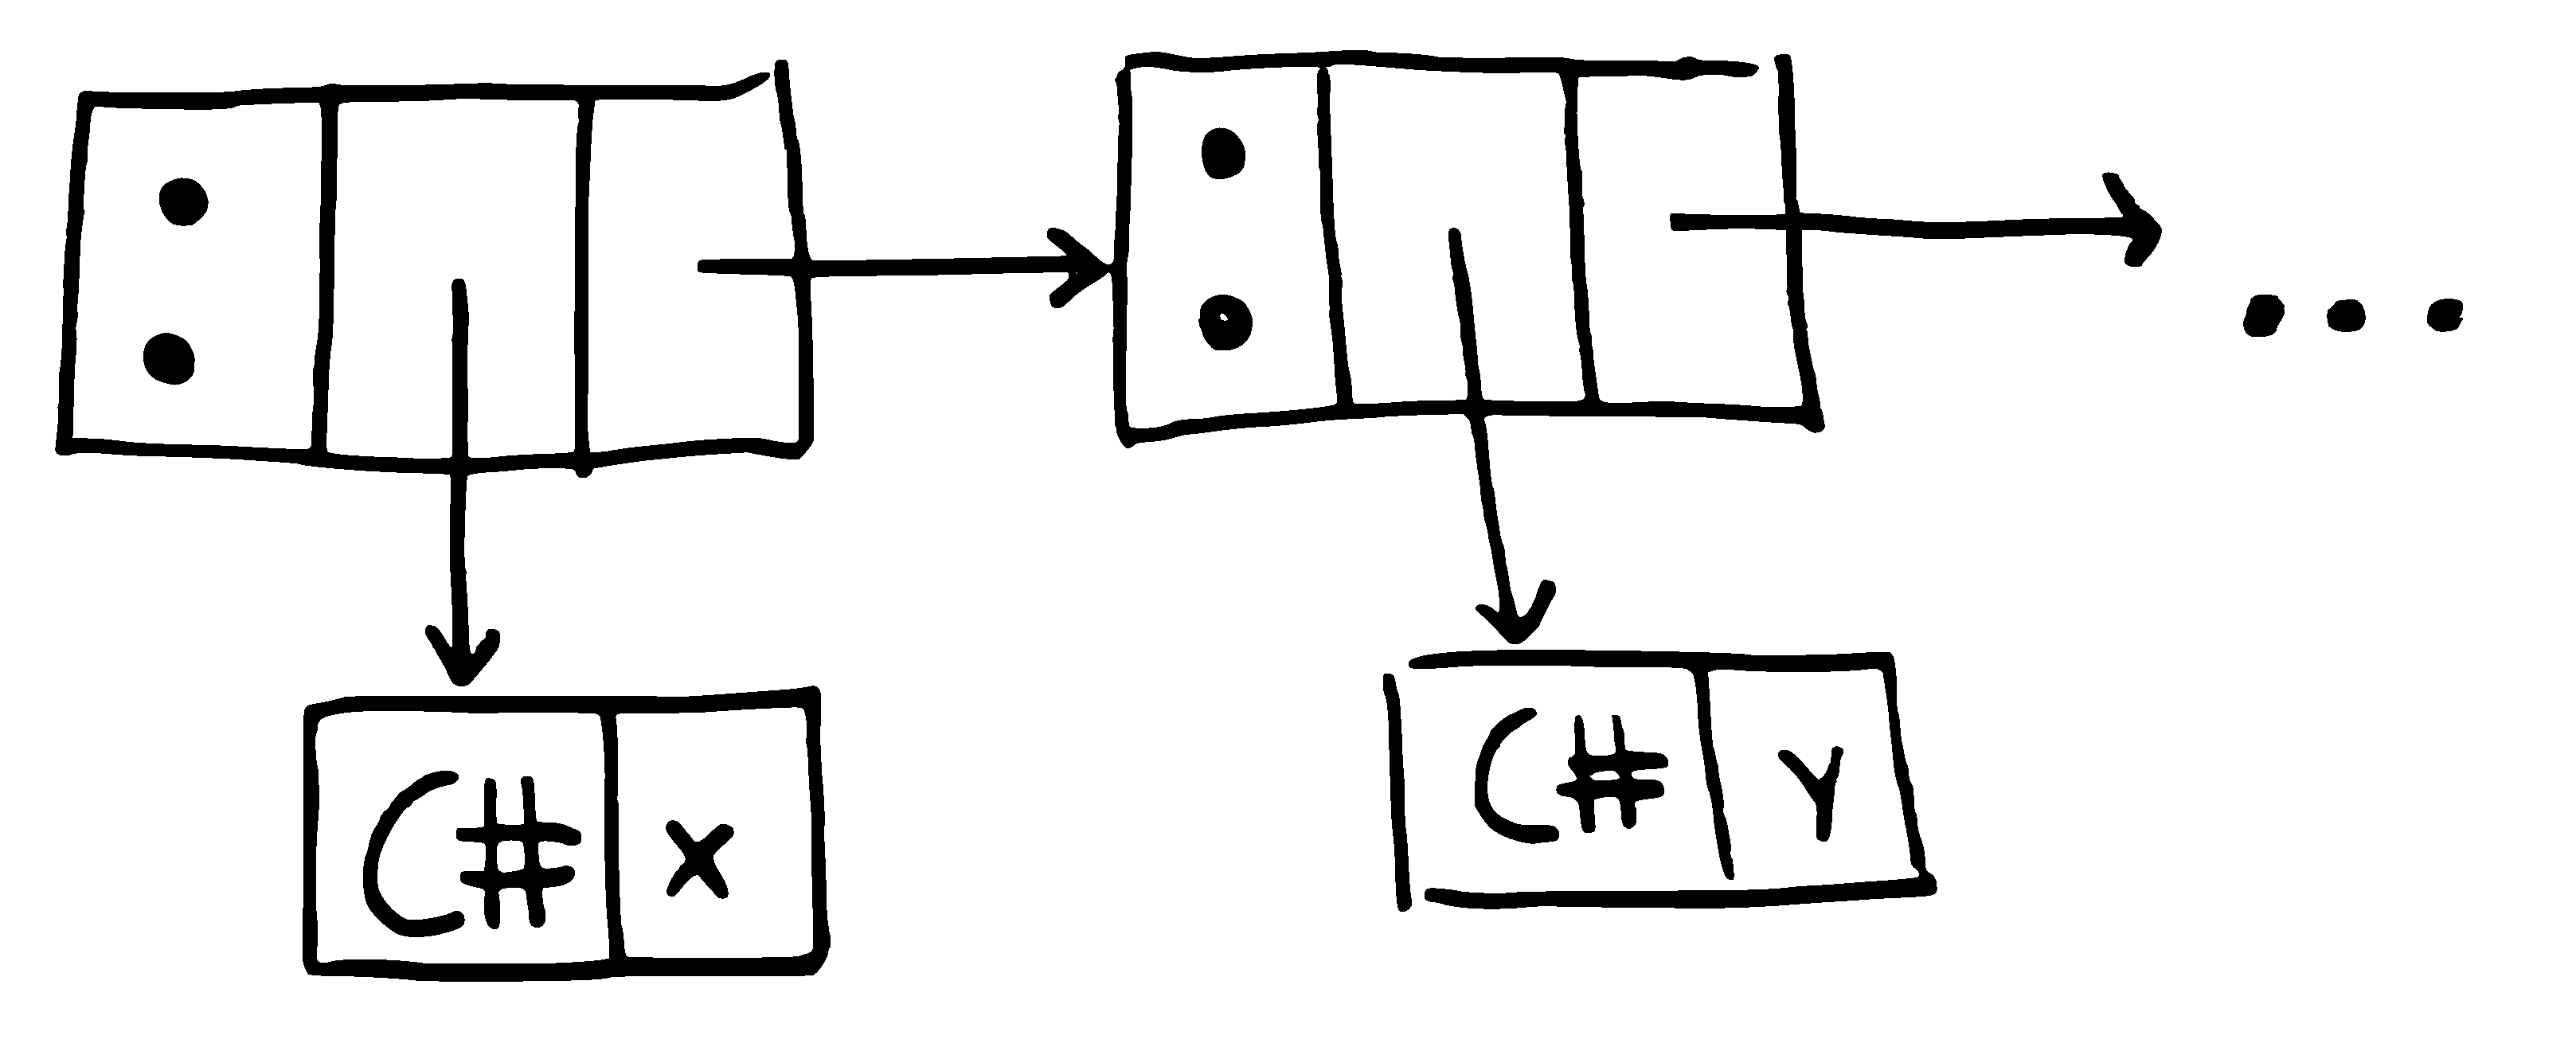
\includegraphics[width=\textwidth]{../2011-dutchhug-text-utf8/images/string.pdf}
    \end{center}
\end{frame}


\begin{frame}{Use \texttt{String} with care}
    Two points: \\
    \begin{enumerate}
    \item Use strict arrays
    \item Don't use a 32-bit encoding
    \end{enumerate}
\end{frame}

% Unicode crash course
% --------------------

\begin{frame}{Overview}
    Introduction \\
    Use \texttt{String} with care \\
    \textbf{Unicode crash course} \\
    Results \\
\end{frame}

\begin{frame}{Unicode crash course}
    \begin{center}
    This is UTF-8 \\
    \vspaced
    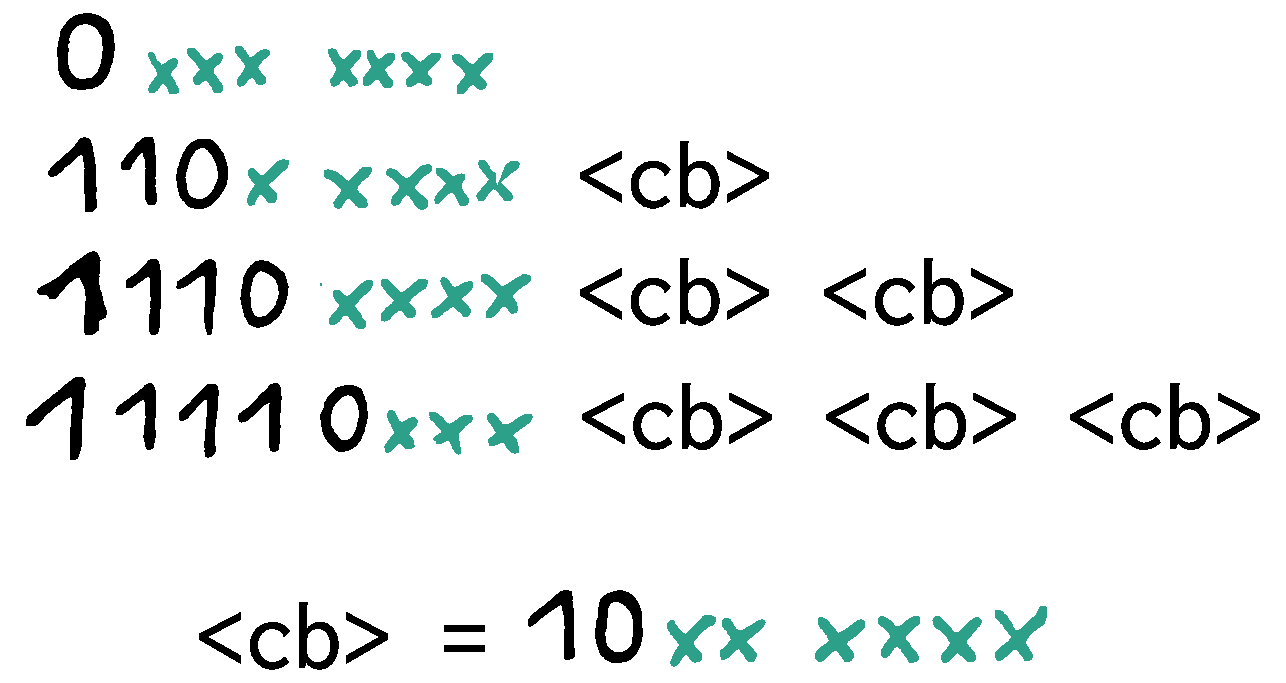
\includegraphics[width=0.9\textwidth]{../2011-dutchhug-text-utf8/images/utf8.pdf}
    \end{center}
\end{frame}

\begin{frame}{Unicode crash course}
    \begin{center}
    This is UTF-16 \\
    \vspaced
    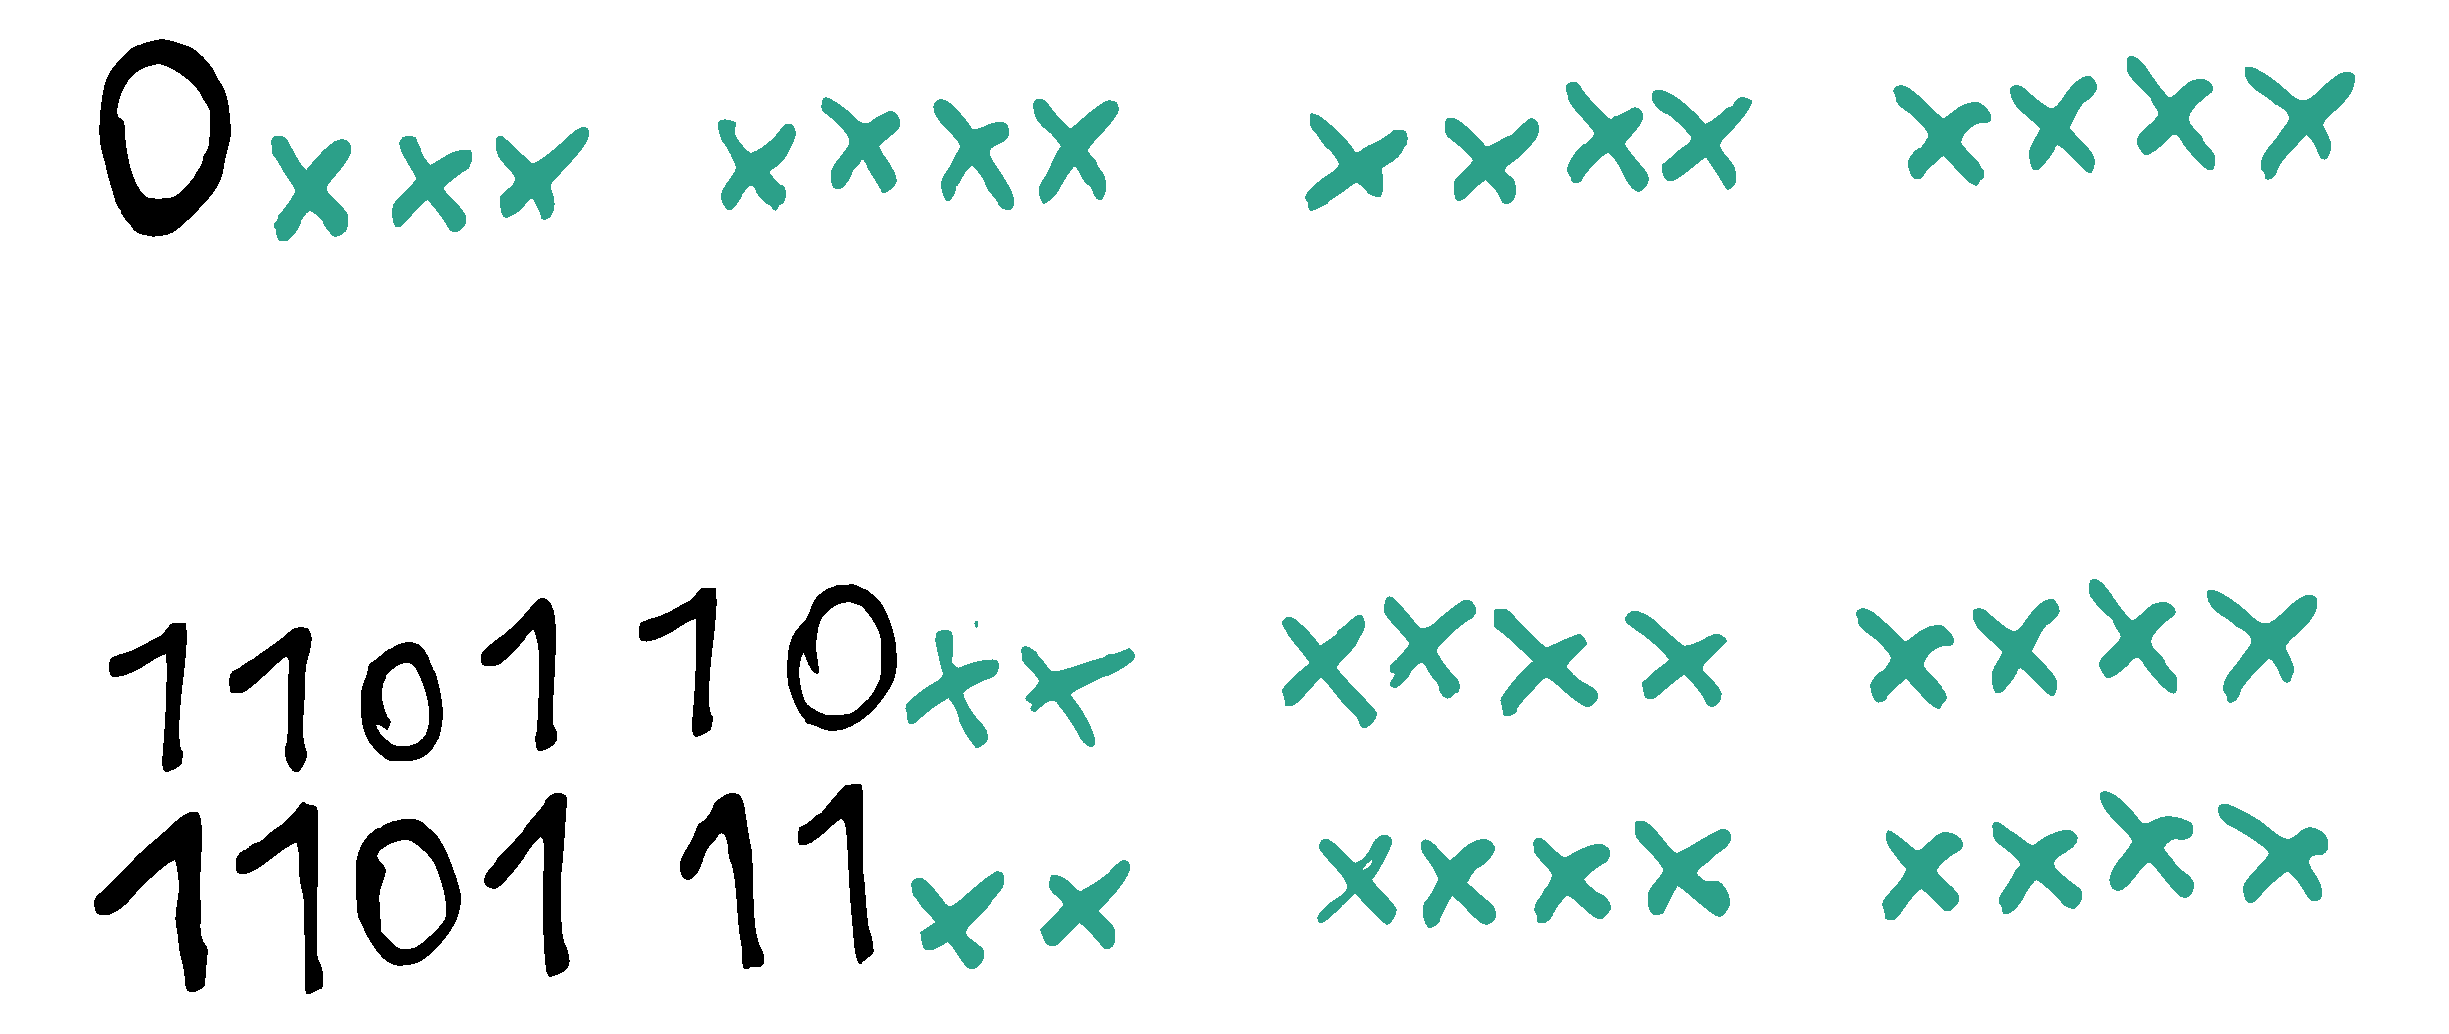
\includegraphics[width=0.9\textwidth]{../2011-dutchhug-text-utf8/images/utf16.pdf}
    \end{center}
\end{frame}

\begin{frame}{Unicode crash course}
    Two points:
    \begin{enumerate}
    \item Some things are inherently faster using UTF-8
    \item Some things are inherently faster using UTF-16
    \end{enumerate}
\end{frame}

\begin{frame}{Unicode crash course}
    Results depend on:
    \begin{enumerate}
    \vspaced
    \item The application (e.g. lots of processing vs. static in-memory
    database)
    \vspaced
    \item The language (e.g. English vs. Japanese)
    \end{enumerate}
\end{frame}

% Results
% -------

\begin{frame}{Overview}
    Introduction \\
    Use \texttt{String} with care \\
    Unicode crash course \\
    \textbf{Results} \\
\end{frame}

\begin{frame}[fragile]{Results: pure functions}
    \begin{lstlisting}
    stream   :: Text -> Stream Char
    unstream :: Stream Char -> Text

    map :: (Char -> Char)
        -> Text -> Text
    map f =
        unstream . map' f . stream
    \end{lstlisting}
\end{frame}

\begin{frame}[fragile]{Results: pure functions}
    \begin{lstlisting}
    map :: (Char -> Char)
        -> Text -> Text
    map f =
        unstream . map' f . stream
    \end{lstlisting}
    \vspaced
    ``\textit{Generally}'' a little slower for UTF-8
\end{frame}

\begin{frame}[fragile]{Results: applications}
    \begin{lstlisting}
    program :: ByteString
            -> ByteString
    program = encodeUtf8
            . map someF
            . decodeUtf8
    \end{lstlisting}
    \vspaced
    ``\textit{Generally}'' a little faster for UTF-8
\end{frame}

\begin{frame}{Results}
    \textbf{Other advantages} \\
    \vspaced
    Integrate with C libraries (e.g. \texttt{pcre}) \\
    Reduced memory usage \\
    Fast output path (for e.g. \texttt{aeson}) \\
\end{frame}

\begin{frame}{Results}
    \textbf{GSoC: progress} \\
    \vspaced
    \begin{tabular}{ll}
    Conversion:     & done \\
    Optimization:   & done* \\
    Summary report: & in progress \\
    Switch:         & ? \\
    \end{tabular}
    \newline
    \newline
    \vspaced
    *\small{\textit{always room for improvement}} \\
\end{frame}

\begin{frame}[plain]
    \begin{center}
    \huge{Questions?}
    \end{center}
\end{frame}

\end{document}
